
\chapter{Elaboración}
\noindent En el presente capítulo se reforzará y se analizará la solución que se planteó en el capítulo anterior teniendo como resultado los siguientes elementos:

\begin{itemize}
\item Diseño de requerimientos
\item Diseño de la base de datos
\item Especificación Plan de pruebas
\item Entorno de Desarrollo
\item Proceso de Integración Continua
\item Plan de Iteraciones 
\end{itemize}

\noindent El objetivo de la fase de \textbf{Elaboración} en AUP - Proceso Unificado Ágil, es que el equipo de desarrollo profundice en la comprensión de los requisito del sistema y en validar la arquitectura propuesta en la fase de \textbf{Iniciación}.

\noindent Adicionalmente en este capítulo se ha considerado los siguientes elementos de la metodología 12 factor:
\begin{itemize}
\item Minimizar tiempo de encendido y apagado aplicación
\item Concurrencia
\item Código Base
\item Dependencias
\item Configuraciones
\end{itemize}

\section{Diseño de requerimientos}
\noindent A continuación de definen los diseños por cada módulo definido en la arquitectura presentada en el capítulo anterior. Para una mejor compresión se define por cada módulo: los diagramas de secuencia, diagramas de clases, diseño de interfaz gráfica y especificación de criterios de aceptación para las pruebas.

\subsection{Módulo de Pedidos}
\noindent El módulo de pedidos tiene como objetivo resolver los siguientes requerimientos:
\begin{itemize}
\item Registro de los pedidos realizados por los clientes (Req. \#1).
\item Asignación de pedidos a los motorizados de la empresa (Req. \#2).
\item Listar los pedidos realizados en el dia (Req \#3).
\end{itemize}

\begin{figure}[H]
  \centering
  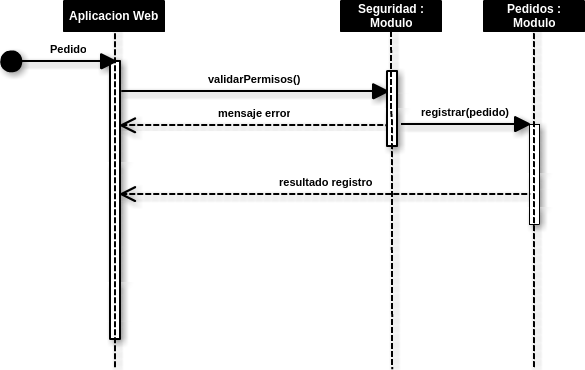
\includegraphics[width=11cm, height=8cm]{chapter4-register-customer-request-sequence-diagram.png}
  \caption{Registro de pedidos [Elaboración propia]}  
\end{figure}

\begin{figure}[H]
  \centering
  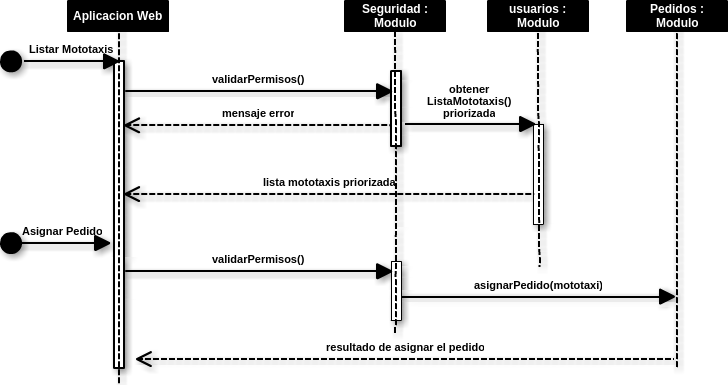
\includegraphics[width=12cm, height=8cm]{chapter4-assign-customer-request-sequence-diagram.png}
  \caption{Asignación de pedidos [Elaboración propia]}  
\end{figure}

\begin{figure}[H]
  \centering
  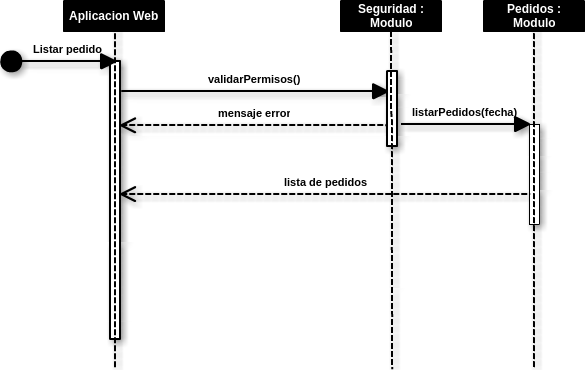
\includegraphics[width=11cm, height=8cm]{chapter4-get-list-customer-request-sequence-diagram.png}
  \caption{Obtener lista de pedidos [Elaboración propia]}  
\end{figure}


\begin{figure}[H]
  \centering
  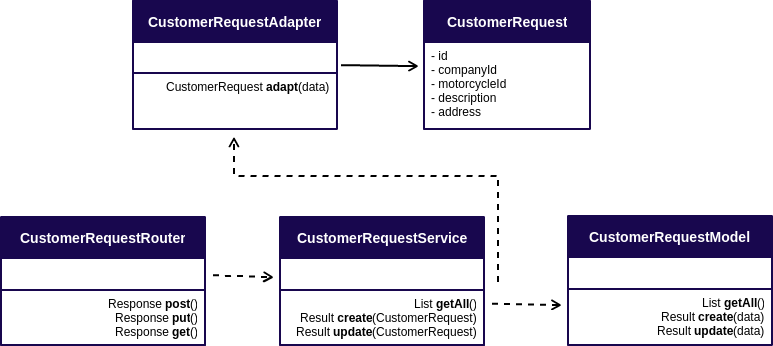
\includegraphics[width=14cm, height=7cm]{chapter4-customer-request-module-class-diagram.png}
  \caption{Diagrama de clases módulo de pedidos [Elaboración propia]}  
\end{figure}

\begin{figure}[H]
  \centering
  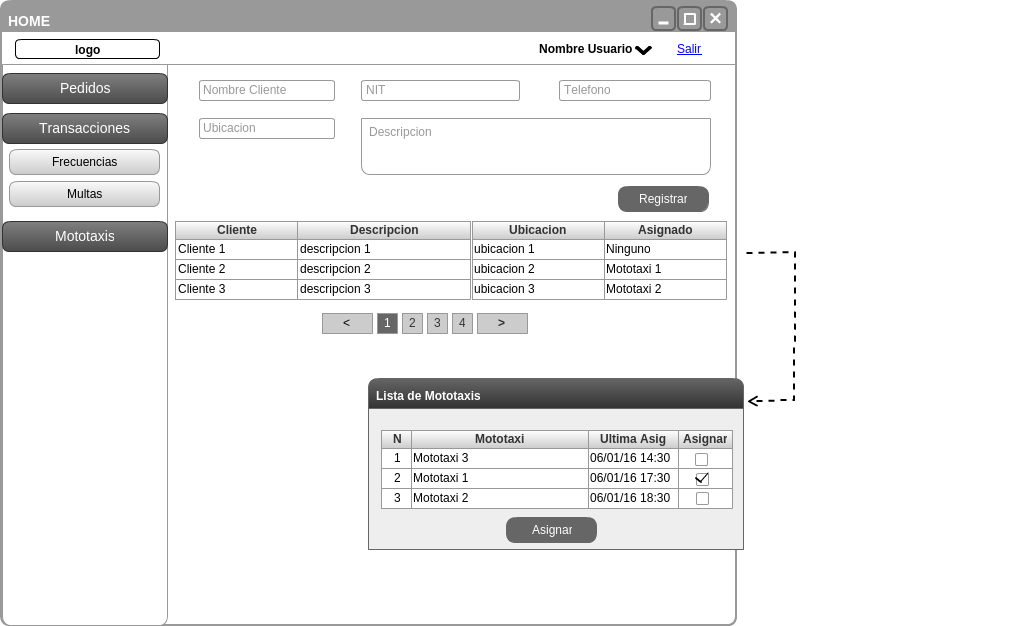
\includegraphics[width=22cm, height=15cm]{chapter4-customer-request-module-view-design.png}
  \caption{Diseño de la vista módulo de pedidos [Elaboración propia]}  
\end{figure}

\subsection{Módulo de Transacciones}
El módulo de transacciones tiene como objetivo resolver los siguientes requerimientos:
\begin{itemize}
\item Registrar el cobro por frecuencia diaria a los respectivos motorizados de la empresa (Req. \#5).
\item Registrar el cobro por multa de inasistencia de los respectivos motorizados de la empresa (Req. \#6).
\end{itemize}
\subsection{Módulo de Usuarios}
El módulo de Usuarios tiene como objetivo resolver los siguientes requerimientos:
\begin{itemize}
\item Registro de motorizados de la respectiva empresa (Req. \#4).
\item Listar los motorizados de la respectiva empresa (Req. \#7).
\item Registro de cuentas de operadores de la respectiva empresa (Req. \#8).
\item Ver ingresos diarios y mensuales de los ingresos por cobro de frecuencia y multas (Req. \#9).
\item Actualizar datos de usuarios (Req. \#10).
\end{itemize}
\subsection{Módulo de Seguridad}
\noindent El módulo de Seguridad tiene como objetivo resolver los siguientes requerimientos:
\begin{itemize}
\item Autenticación de usuarios y mostrar la información de acuerdo al perfil usuario (Req. \#11).
\item Control permisos de accesos a los recursos de información de acuerdo al perfil de usuario (Req. \#12).
\item Control de acceso a los usuarios que solo puedan acceder a la información de la empresa a la cual pertenecen (Req. \#13).
\item Permitir crear solo una cuenta administrador por empresa (Req. \#14).
\item Permitir cambiar contraseña (Req. \#15).
\end{itemize}

\section{Diseño de la base de datos}
\noindent Para el diseño de la base de datos se ha considerado las sugerencias descritas en [mongoDB data model design, 2014] para la elaboración de un modelo de datos en mongodb donde se puede tener modelos de datos embebidos y/o modelo de datos normalizados.

\noindent La estructura de una base de datos en mongodb está compuesta por las colecciones (tablas sql). En una colecciones se almacenan los documentos (filas sql), los documentos son objetos en formato json que almacenan la información en clave-valor.

\begin{figure}[H]
  \centering
  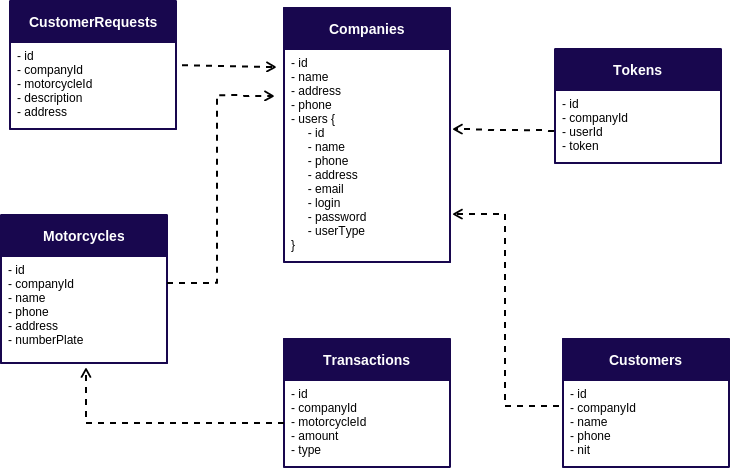
\includegraphics[width=14cm, height=8cm]{chapter4-database-design.png}
  \caption{Colecciones de la base de datos [Elaboración propia]}  
\end{figure}

\section{Entorno de Desarrollo}

\section{Proceso de Integración Continua}

\section{Plan de Iteraciones}

 
